\documentclass[tikz, border=14pt]{standalone}
\usepackage{tikz}
\usetikzlibrary{arrows.meta, positioning, calc, backgrounds, fit}
\usepackage{amsmath}

% ── Palette ────────────────────────────────────────────────────────────
\colorlet{cTrain}{green!22!white}
\colorlet{cFrozen}{blue!18!white}
\colorlet{cInput}{gray!10!white}
\colorlet{cLoss}{orange!28!white}

% ── Node styles ────────────────────────────────────────────────────────
\tikzset{
  block/.style  = {draw, rounded corners=3pt,
                   minimum width=4.0cm, minimum height=0.72cm,
                   align=center, inner sep=5pt, font=\small},
  inp/.style    = {block, fill=cInput,   draw=gray!60},
  trn/.style    = {block, fill=cTrain,   draw=black!70},
  frz/.style    = {block, fill=cFrozen,  draw=blue!50!black},
  lss/.style    = {block, fill=cLoss,    draw=orange!70!black},
  arr/.style    = {-{Stealth[length=2.8pt, width=2.2pt]},
                   line width=0.9pt},
  det/.style    = {arr, dashed, gray!70},
  lbl/.style    = {font=\scriptsize, fill=white,
                   inner sep=1.5pt, midway},
  side/.style   = {arr, gray!60},
}

\begin{document}
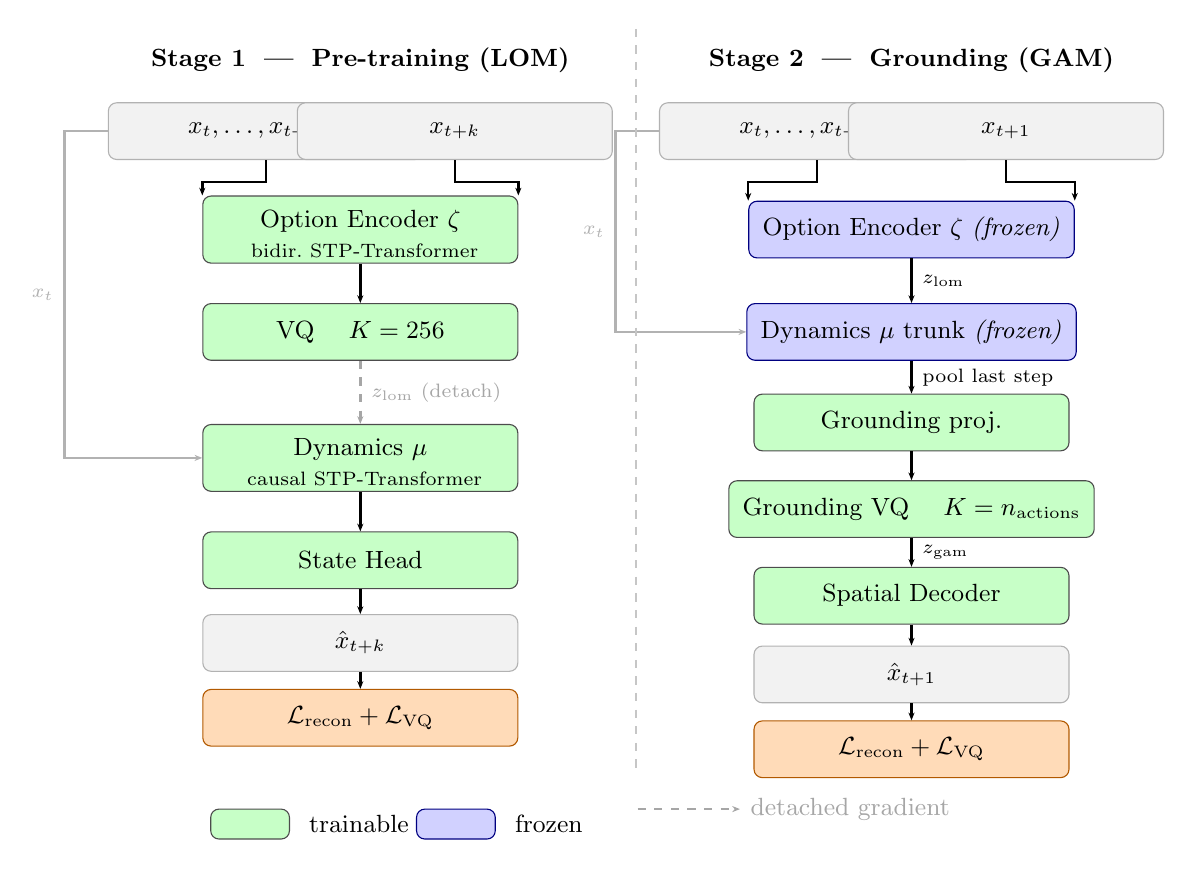
\begin{tikzpicture}

%% ════════════════════════════════════════════════════════════════
%%  STAGE 1 — Pre-training  (left column, x-centre = 2 cm)
%% ════════════════════════════════════════════════════════════════

\node[font=\small\bfseries] (T1) at (2, 0.5)
  {Stage 1 \;—\; Pre-training (LOM)};

% Inputs
\node[inp] (s1_h)  at (0.8, -0.4)  {$x_t,\ldots,x_{t+c-1}$};
\node[inp] (s1_f)  at (3.2, -0.4)  {$x_{t+k}$};

% Encoder + VQ  (both trainable, shown separately to highlight VQ bottleneck)
\node[trn] (s1_enc) at (2,  -1.65)
  {Option Encoder $\zeta$\\\vspace{-3pt}
   \scriptsize bidir.\ STP-Transformer};

\node[trn] (s1_vq) at (2, -2.95)   {VQ \quad $K=256$};

% Dynamics (receives history directly + z_lom detached)
\node[trn] (s1_dyn) at (2, -4.55)
  {Dynamics $\mu$\\\vspace{-3pt}
   \scriptsize causal STP-Transformer};

\node[trn] (s1_hd) at (2, -5.85)   {State Head};
\node[inp] (s1_out) at (2, -6.90)  {$\hat{x}_{t+k}$};
\node[lss] (s1_loss) at (2, -7.85)
  {$\mathcal{L}_{\mathrm{recon}} + \mathcal{L}_{\mathrm{VQ}}$};

% ── arrows ──
\draw[arr] (s1_h.south) -- ++(0,-0.28) -| (s1_enc.north west);
\draw[arr] (s1_f.south) -- ++(0,-0.28) -| (s1_enc.north east);
\draw[arr] (s1_enc) -- (s1_vq);
\draw[det] (s1_vq)  -- node[lbl, right=2pt]{$z_{\mathrm{lom}}$ (detach)} (s1_dyn);
% history side-feeds dynamics
\draw[side] (s1_h.west) -- ++(-0.55,0)
            |- node[lbl, left=2pt, pos=0.25]{$x_t$} (s1_dyn.west);
\draw[arr] (s1_dyn)  -- (s1_hd);
\draw[arr] (s1_hd)   -- (s1_out);
\draw[arr] (s1_out)  -- (s1_loss);


%% ════════════════════════════════════════════════════════════════
%%  STAGE 2 — Grounding  (right column, x-centre = 9 cm)
%% ════════════════════════════════════════════════════════════════

\node[font=\small\bfseries] (T2) at (9, 0.5)
  {Stage 2 \;—\; Grounding (GAM)};

% Inputs (horizon=1)
\node[inp] (s2_h) at (7.8, -0.4)   {$x_t,\ldots,x_{t+c-1}$};
\node[inp] (s2_f) at (10.2, -0.4)  {$x_{t+1}$};

% Frozen LOM blocks (encoder already contains its VQ)
\node[frz] (s2_enc) at (9, -1.65)
  {Option Encoder $\zeta$ \textit{(frozen)}};

\node[frz] (s2_dyn) at (9, -2.95)
  {Dynamics $\mu$ trunk \textit{(frozen)}};

% Trainable grounding stack
\node[trn] (s2_prj) at (9, -4.10)  {Grounding proj.};
\node[trn] (s2_gvq) at (9, -5.20)
  {Grounding VQ \quad $K=n_{\mathrm{actions}}$};
\node[trn] (s2_dec) at (9, -6.30)  {Spatial Decoder};
\node[inp] (s2_out) at (9, -7.30)  {$\hat{x}_{t+1}$};
\node[lss] (s2_loss) at (9, -8.25)
  {$\mathcal{L}_{\mathrm{recon}} + \mathcal{L}_{\mathrm{VQ}}$};

% ── arrows ──
\draw[arr] (s2_h.south) -- ++(0,-0.28) -| (s2_enc.north west);
\draw[arr] (s2_f.south) -- ++(0,-0.28) -| (s2_enc.north east);
\draw[arr] (s2_enc) -- node[lbl, right=2pt]{$z_{\mathrm{lom}}$} (s2_dyn);
\draw[side] (s2_h.west) -- ++(-0.55,0)
            |- node[lbl, left=2pt, pos=0.25]{$x_t$} (s2_dyn.west);
\draw[arr] (s2_dyn) -- node[lbl, right=2pt]{\scriptsize pool last step} (s2_prj);
\draw[arr] (s2_prj) -- (s2_gvq);
\draw[arr] (s2_gvq) -- node[lbl, right=2pt]{$z_{\mathrm{gam}}$} (s2_dec);
\draw[arr] (s2_dec) -- (s2_out);
\draw[arr] (s2_out) -- (s2_loss);


%% ════════════════════════════════════════════════════════════════
%%  Column divider
%% ════════════════════════════════════════════════════════════════
\draw[thick, dashed, gray!45] (5.5, 0.9) -- (5.5, -8.55);


%% ════════════════════════════════════════════════════════════════
%%  Legend
%% ════════════════════════════════════════════════════════════════
\begin{scope}[shift={(0.6, -9.2)}]
  \node[trn, minimum width=1.0cm, minimum height=0.38cm] (lg_t) {};
  \node[right=0.12cm of lg_t, font=\small] {trainable};

  \node[frz, minimum width=1.0cm, minimum height=0.38cm,
        right=1.6cm of lg_t] (lg_f) {};
  \node[right=0.12cm of lg_f, font=\small] {frozen};

  \draw[det, line width=1pt] ($(lg_f.east) + (1.8, 0.19)$)
    -- ++(1.3, 0) node[right, font=\small] {detached gradient};
\end{scope}

\end{tikzpicture}
\end{document}
